This process is essential to be taken when building an application. This involves designing the front-end as well as a back-end system. This section will explain the design process for each part of the system such as system requirement, wireframe, use case diagram, and more.

\section{System Requirement}
This section will give a better understanding of what the system needs to handle to make a good application. This will be done by making a functional, non-functional, Database, and PHP requirement.

\subsection{Functional Requirement}
\begin{enumerate}
    \item The website must able to run on every single browser that is currently in the market.
    \item The website should be able to display all the products that are in the database.
    \item It should able to show real data in the chart.
    \item The website should able to search the data using the search functionality.
    \item The website should able to add products and display in real-time.
    \item The site should able to delete and edit data in real-time.
    \item The site should able to contact the developer using the contact form.
    \item Users should able to log in and create new users.
    \item Enable easy navigation around the website.
\end{enumerate}

\subsection{Non-Functional Requirement}
\begin{enumerate}
    \item The system should respond quickly to user input such as users want to find a specific product using the search functionality.
    \item The website should have a simple layout with good color.
    \item During the research, I have found that the user does not like too much text on the homepage.
    \item The system will require an internet connection, in order to load up the website and get data from the database.
    \item Ensuring the current data in the database cannot be accessed by unauthorised users.
\end{enumerate}

\subsection{Database Requirement}
\begin{enumerate}
    \item Must able to store the data without redundancy.
    \item Allow quick and easy recovery when needed.
    \item The database system able to delete or update when it is performed by the user form.
\end{enumerate}

\subsection{PHP Requirement}
\begin{enumerate}
    \item The system should able to handle multiple requests from the users.
    \item Must able to perform POST and GET methods.
    \item Must perform the update and delete data from the database.
    \item User's password must be encrypted.
    \item The system must able to track down the unusual activity in the database.
\end{enumerate}

\section{Use Case Diagram}
The use case diagram is very important because it analyse the life cycle of a user when they use the application. The use case diagram(Figure 3.1) deals with three different scenarios where users search product, edit product, and contact us form. First scenarios where a user searches the product, they need to enter the item number or item name where the server receives that input and find all the records which will be displayed backed to the user browser. Second scenarios, users want to edit the existing record where a user clicks on the edit button which will take them to edit form and update the record from the database. Final scenarios where a user wants to send a message using the form on the contact page. Once the form is submitted, the server process the message using the telegram API and displays it in the telegram app.

\begin{figure}[h]
\centering
    \includegraphics[scale=0.55]
    {Diagrams/usecasediagram.png}
    \caption{Use Case Diagram}
    \label{fig:Use case diagram}
\end{figure}

\section{Wireframe}
This part plays a big role in the user interface and experience when the user visits my site. My aims are to make the website simple and easy to navigate without any problems because some of the shopkeepers may not able to use the system if the UI is complicated to use. Therefore I have asked my uncle what kind of interface he was looking for and he said: "simple and easy to manage everyday inventory". The first mission was to find what interface is currently looking in other inventory systems and make a difference to them. Furthermore, it will fail the design if the UI is complex.\newline
\newline I have created two different wireframes using an online tool(wireframe.cc). The first wireframe (Figure 3.2, 3.3, 3.4 3.5) was designed and taken backed to my uncle to gain feedback and allow me to improve them if there is something missing in the UI. The second wireframe was designed with the improvement that was suggested by my uncle.  

\subsection{Wireframe 1}
\begin{figure}[h]
\centering
    \includegraphics[scale=0.37]
    {wireframe1/HomePage.png}
    \caption{Wireframe 1 - Homepage}
    \label{fig:Wireframe 1 - Homepage}
\end{figure}

\begin{figure}[H]
\centering
    \includegraphics[scale=0.37]
    {wireframe1/Product.png}
    \caption{Wireframe 1 - Product}
    \label{fig:Wireframe 1 - product}
\end{figure}

\begin{figure}[H]
\centering
    \includegraphics[scale=0.37]
    {wireframe1/Analystic.png}
    \caption{Wireframe 1 - Analystic}
    \label{fig:Wireframe 1 - Analystic}
\end{figure}

\begin{figure}[H]
\centering
    \includegraphics[scale=0.5]
    {wireframe1/contactus.png}
    \caption{Wireframe 1 - Contact us}
    \label{fig:Wireframe 1 - Contact us}
\end{figure}

\subsection{Wireframe 2}
The wireframe 2 is the final UI which you will see on the actual website. To get the review of the design, shown this to my uncle and other shopkeeper and they were impressed with the design of the application.
\begin{figure}[H]
\centering
    \includegraphics[scale=0.4]
    {wireframe2/homepage2.png}
    \caption{Wireframe 2 - Homepage}
    \label{fig:Wireframe 2 - Homepage}
\end{figure}

Figure 3.7, below page open up and asked user to click on view all product or add product button. 
\begin{figure}[H]
\centering
    \includegraphics[scale=0.5]
    {wireframe2/product2.png}
    \caption{Wireframe 2 - Product}
    \label{fig:Wireframe 2 - Product}
\end{figure}

Figure 3.8, below page open up when the user click on view all product from the product page. 
\begin{figure}[H]
\centering
    \includegraphics[scale=0.5]
    {wireframe2/viewallproduct.png}
    \caption{Wireframe 2 - View all product}
    \label{fig:Wireframe 2 - view all product}
\end{figure}

\newpage
Figure 3.9, below page open up when the user click on add product from the product page. 
\begin{figure}[H]
\centering
    \includegraphics[scale=0.5]
    {wireframe2/addproduct.png}
    \caption{Wireframe 2 - Add product}
    \label{fig:Wireframe 2 - Add  product}
\end{figure}

Figure 3.10, below page open up when the user click on edit button from view all product page. 
\begin{figure}[H]
\centering
    \includegraphics[scale=0.5]
    {wireframe2/editproduct.png}
    \caption{Wireframe 2 - Edit product}
    \label{fig:Wireframe 2 - Edit  product}
\end{figure}

\begin{figure}[H]
\centering
    \includegraphics[scale=0.5]
    {wireframe2/Analystic2.png}
    \caption{Wireframe 2 - Analystic}
    \label{fig:Wireframe 2 - Analystic}
\end{figure}

\begin{figure}[H]
\centering
    \includegraphics[scale=0.5]
    {wireframe2/contactus2.png}
    \caption{Wireframe 2 - Contact us}
    \label{fig:Wireframe 2 - contact us}
\end{figure}
 
\newpage
\subsection{Final outcome}
The following images are the final UI that was implemented after finalising the wireframe 2. The UI was made with the right choice of color, Scale and compatible with mobile browser.\newline
\newline Figure 3.13 is the main page of the website where the user can log in to the account and also create the account if they have not made one. This feature is currently not available at the moment but will my implemented in the feature.

\begin{figure}[h]
\centering
    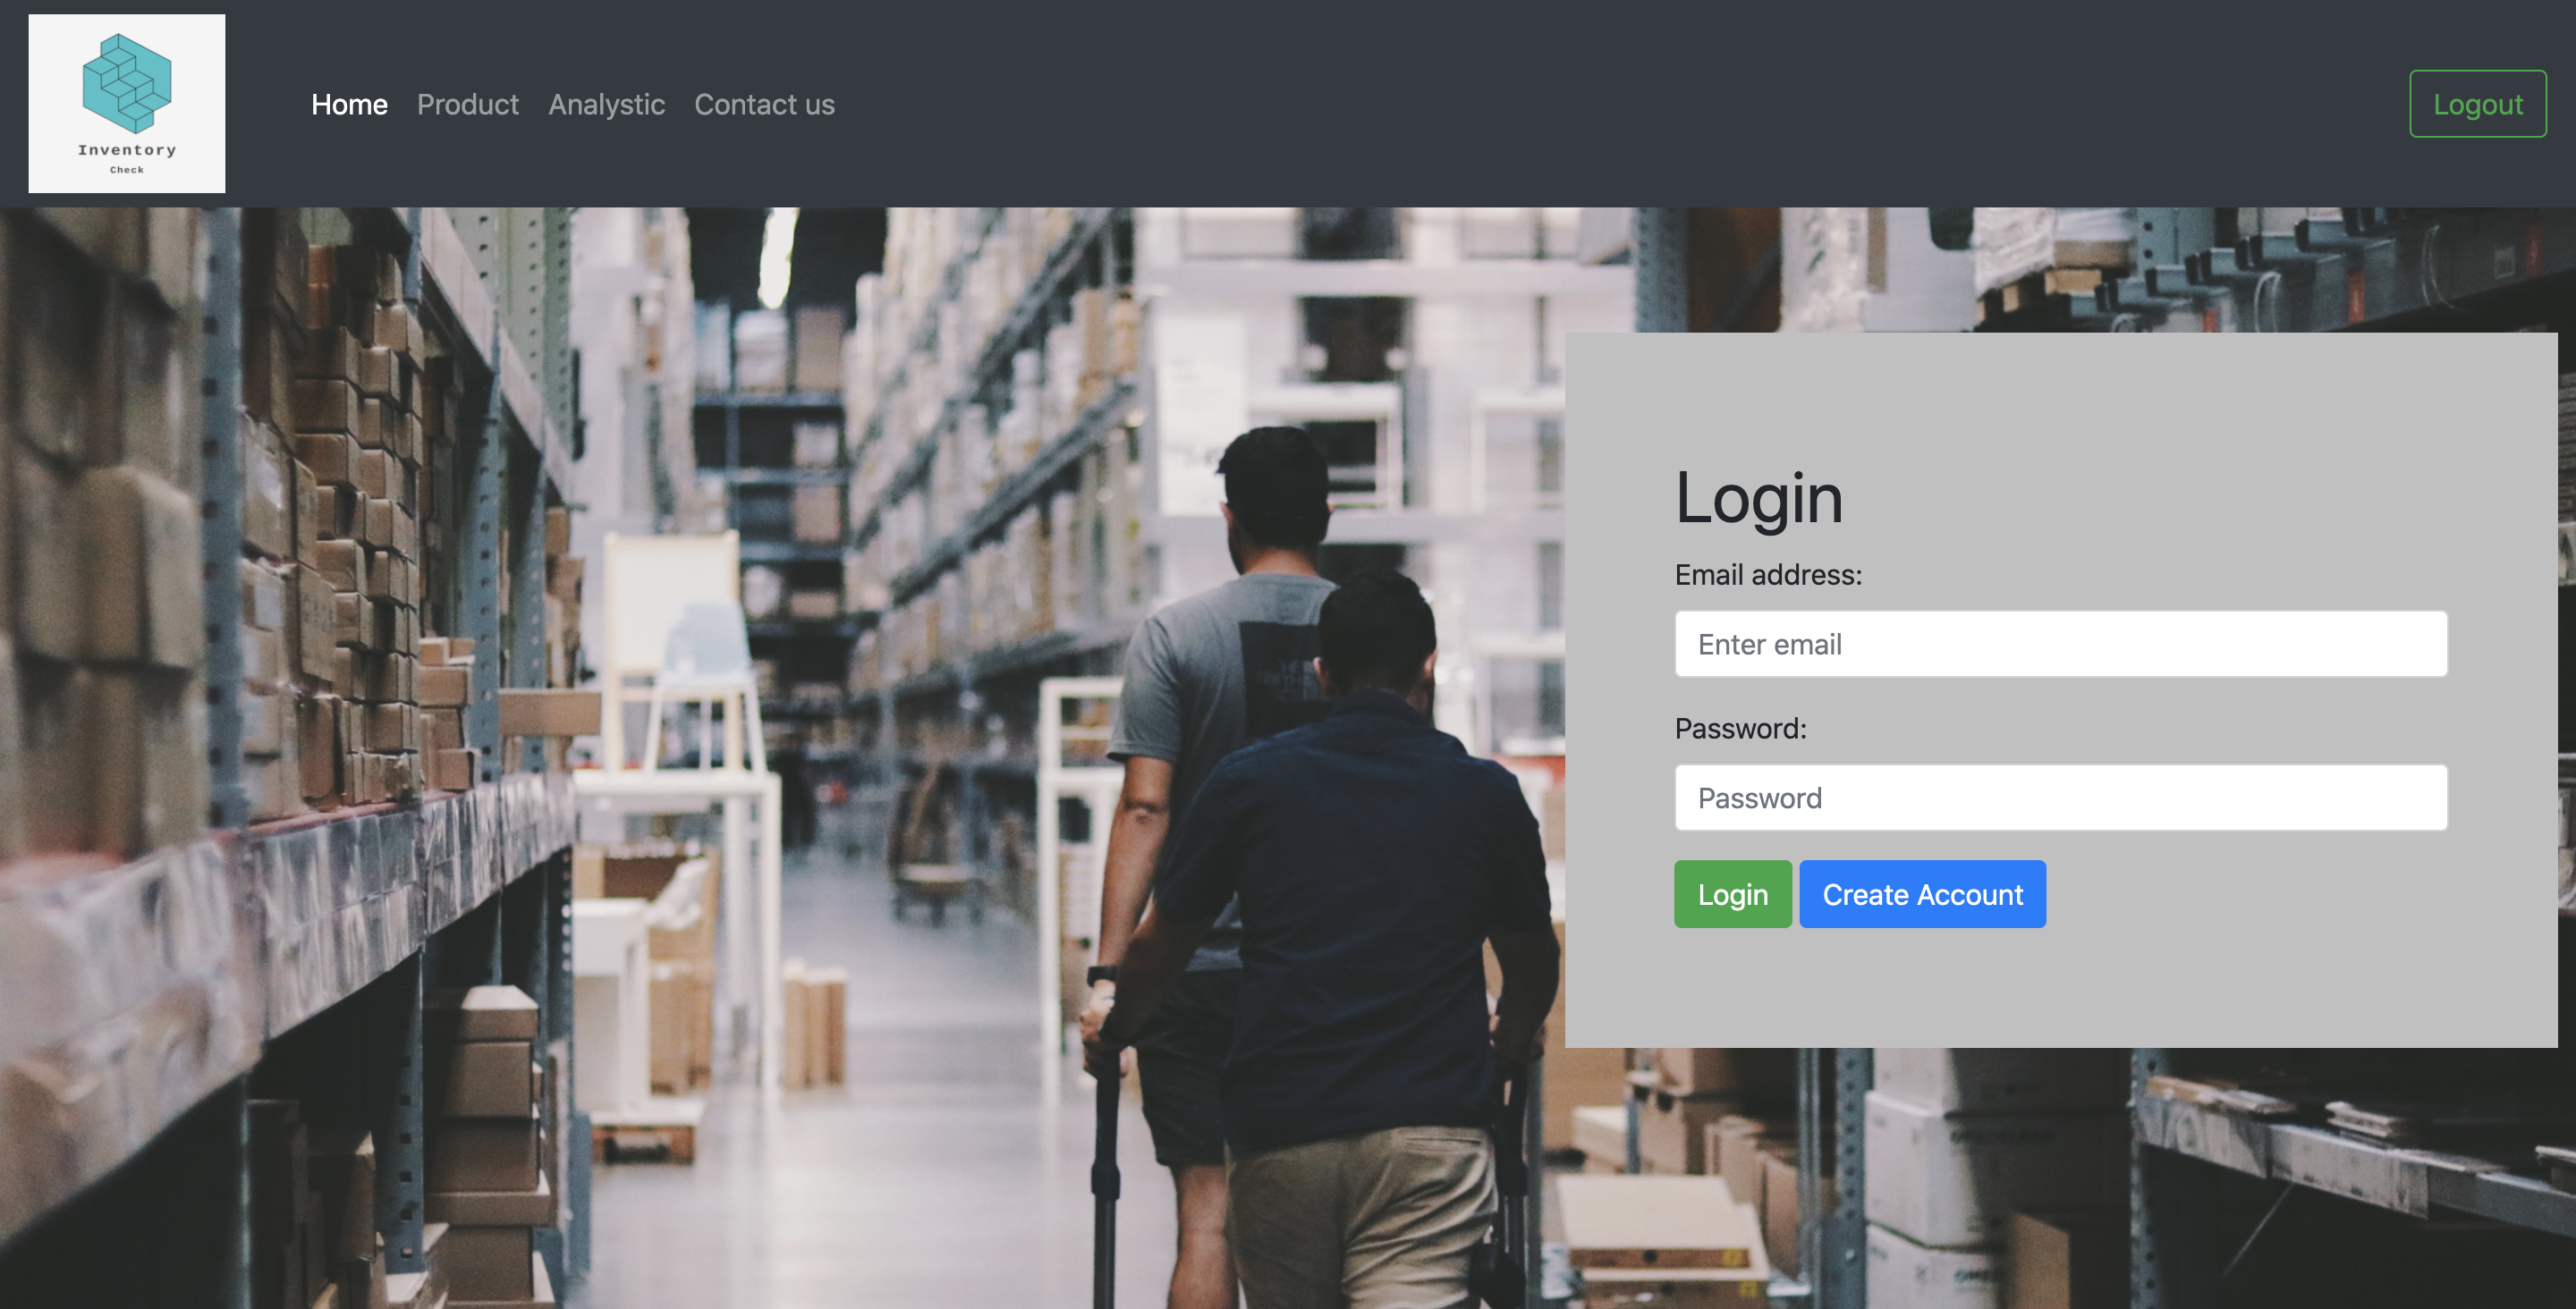
\includegraphics[scale=0.27]
    {FinalUI/homepage.png}
    \caption{Final UI - Homepage}
    \label{fig:Final UI - Homepage}
\end{figure}

\newpage
Figure 3.14 is the product where user can select view all product or add product model which will take them to there destination. 
\begin{figure}[H]
\centering
    \includegraphics[scale=0.27]
    {FinalUI/product.png}
    \caption{Final UI - Product}
    \label{fig:Final UI - product}
\end{figure}

Figure 3.15 is the view all product where user can view all the product that are stored in the database, edit the item, delete the item and search for specific product using item name or item number.
\begin{figure}[H]
\centering
    \includegraphics[scale=0.27]
    {FinalUI/viewallproduct.png}
    \caption{Final UI - View all product}
    \label{fig:Final UI - view all product}
\end{figure}

Figure 3.16 is the UI of search result when user search the product from view all product page.
\begin{figure}[H]
\centering
    \includegraphics[scale=0.27]
    {FinalUI/search.png}
    \caption{Final UI - Search Result}
    \label{fig:Final UI - Search Result}
\end{figure}

Figure 3.17 is the edit form where user can update the product that are stored in the database.
\begin{figure}[H]
\centering
    \includegraphics[scale=0.3]
    {FinalUI/editproduct.png}
    \caption{Final UI - Edit Product}
    \label{fig:Final UI - Edit Product}
\end{figure}

Figure 3.18 where user can add product in the database and view the product in the product page once it has been successful stored in the database.
\begin{figure}[H]
\centering
    \includegraphics[scale=0.27]
    {FinalUI/addproduct.png}
    \caption{Final UI - Add Product}
    \label{fig:Final UI - Add Product}
\end{figure}

\begin{figure}[H]
\centering
    \includegraphics[scale=0.27]
    {FinalUI/analystic.png}
    \caption{Final UI - Analystic}
    \label{fig:Final UI - Analystic}
\end{figure}

\begin{figure}[H]
\centering
    \includegraphics[scale=0.24]
    {FinalUI/contactus.png}
    \caption{Final UI - Contact us}
    \label{fig:Final UI - Contact us}
\end{figure}

\section{Side Map}
It is a list of pages that are on the website. By making this diagram, it shows the developer where/how all the pages are linked together across the site.

\begin{figure}[H]
\centering
    \includegraphics[scale=0.52]
    {Diagrams/sidemap.png}
    \caption{Side Map}
    \label{fig:Side map}
\end{figure}